%%%%%%%%%%%%%%%%%%%%%%%%%%%%%%%%%%%%%%%%%%%%%%%%%%
%%%%		~~~~ EDITOR'S NOTE ~~~~
%%%%%%%%%%%%%%%%%%%%%%%%%%%%%%%%%%%%%%%%%%%%%%%%%%
%
% This is a template for the Applied Data Science master project
%
% This document is inteded to be a style guide to a nice and fancy LaTeX thesis.
%			- Comments are used to explain code (% sign)
%			- Make it your own by selecting only the things you want
%
% The documents is made of parts, which can be found in the different folders 
%
%%%%%%%%%%%%%%%%%%%%%%%%%%%%%%%%%%%%%%%%%%%%%%%%%%
%%%%	 	 ~~~~ END OF: EDITOR'S NOTE ~~~~
%%%%%%%%%%%%%%%%%%%%%%%%%%%%%%%%%%%%%%%%%%%%%%%%%%


%%%%%%%%%%%%%%%%%%%%%%%%%%%%%%%%%%%%%%%%%%%%%%%%%%
%%%%		~~~~ PREAMBLE ~~~~
%%%%%%%%%%%%%%%%%%%%%%%%%%%%%%%%%%%%%%%%%%%%%%%%%%
 
% SET DOCUMENT CLASS, PAGE SETTINGS, FONT...
\documentclass[12pt,a4paper,twoside,openany,justified]{book}

% SET FONT TYPE
\usepackage[T1]{fontenc}
\usepackage{mathpazo}
% OTHER FONTS....
% \usepackage[libertine,cmintegrals,cmbraces,vvarbb]{newtxmath}
% \usepackage{tgpagella}
% \usepackage{lmodern}

% LOAD PACKAGES, DETAILS EXPLAINED THERE!
%%%%%%%%%%%%%%%%%%%%%%%%%%%%%%%%%%%%%%%%%%%%%%%%%%
%%%%		~~~~ PACKAGE LISTING ~~~~
%%%%%%%%%%%%%%%%%%%%%%%%%%%%%%%%%%%%%%%%%%%%%%%%%%


% USED TO SET TEMPORARY TEXT
\usepackage{lipsum}

% neater appendix
\usepackage{appendix}

% Nicer ragged edges
\usepackage[document]{ragged2e}

% better representation of figures
\usepackage{graphicx}

% language packages & linebreaking
\usepackage[english]{babel}

% Computer science style quotes
\usepackage{csquotes}

% Makes Natbib and hyperref work together
\usepackage{hyphenat}

% slightly different styling of abstract
\usepackage{bookabstract}

% ADJUSTABLE BOXES
\usepackage{adjustbox}

% FOR USING LANDSCAPE PAGES
\usepackage{lscape}


% Filling out the text
\usepackage[parfill]{parskip}
\setlength\parskip{.5\baselineskip plus .1\baselineskip minus .1\baselineskip}



%%%%%%%%%%%%%%%%%%%%%%%%%%%%%%%%%%%%%%%%%%%%%%%%%%
%%%%		~~~~ GEOMETRY STYLE ~~~~
%%%%%%%%%%%%%%%%%%%%%%%%%%%%%%%%%%%%%%%%%%%%%%%%%%

% MAKE ALL THE TEXT JUSTIFIED
\usepackage{ragged2e}
\justifying

% SET PAGE MARGINS
\usepackage[top=30mm, bottom=30mm, inner=35mm, outer=35mm, headsep=10mm, footskip=12mm]{geometry}

% INCREASES THE SPACE BETWEEN LINES, EASIER READABILITY
\usepackage{setspace}
\setstretch{1.4}


% SET MAXIMUM DEPTH OF TOC AND SECTIONS
\setcounter{secnumdepth}{4}
\setcounter{tocdepth}{1}

% SET SPACE BETWEEN TEXT AND FOOTNOTES
\setlength{\skip\footins}{8mm}

% SET PARAGRAPH INDENT
\setlength{\parindent}{0pt}
\setlength{\parskip}{2mm}

% This removes the forced empty pages
\let\cleardoublepage\clearpage


%%%%%%%%%%%%%%%%%%%%%%%%%%%%%%%%%%%%%%%%%%%%%%%%%%
%%%%		~~~~ HEADER STYLING ~~~~
%%%%%%%%%%%%%%%%%%%%%%%%%%%%%%%%%%%%%%%%%%%%%%%%%%

\addtolength{\headheight}{3pt}
\usepackage{fancyhdr}
\pagestyle{fancy}% <- must be used before the redefinition of \chaptermark and \sectionmark
% change the marks set by \chapter and \section
\renewcommand{\chaptermark}[1]{\markboth{#1}{}}
\renewcommand{\sectionmark}[1]{\markright{\thesection\ #1}}

% change fancy style
\fancypagestyle{fancy}{%
\fancyhf{}
\fancyhead[LE]{\nouppercase{\leftmark}}
\fancyhead[RO]{\nouppercase{\rightmark}}
\fancyfoot[RE,RO]{\thepage}
\renewcommand{\headrulewidth}{0.4pt}
}

% change plain style
\fancypagestyle{plain}{%
\fancyhf{}
% \fancyhead[LE]{\nouppercase{\leftmark}}
% \fancyhead[RO]{\nouppercase{\rightmark}}
\fancyfoot[RE,RO]{\thepage}
\renewcommand{\headrulewidth}{0pt}
}

% PAGESTYLE IN TOC
\fancypagestyle{toc}{%
  \fancyhf{}
  \fancyfoot[RE,RO]{\thepage}
}

%%%%%%%%%%%%%%%%%%%%%%%%%%%%%%%%%%%%%%%%%%%%%%%%%%
%%%%		~~~~ BIBLIOGRAPHY STYLE CHOICES ~~~~
%%%%%%%%%%%%%%%%%%%%%%%%%%%%%%%%%%%%%%%%%%%%%%%%%%

% BIBLIOGRAPHY STYLE 
\usepackage[
    backend=biber,
    style=ieee,
    sorting=none,
  ]{biblatex}
\addbibresource{bibliography.bib}

% MANAGE LONG BIBLIOGRAPHY URL
\setcounter{biburlnumpenalty}{9000}
\setcounter{biburlucpenalty}{9000}
\setcounter{biburllcpenalty}{9000}


% SET CHAPTER APPEARENCE (ADD NUMBER NEXT TO THE CHAPTER, MARGIN...)
\usepackage{titlesec}
\titleformat{\chapter}[hang]{\LARGE\bfseries}{\thechapter{. }}{0pt}{\LARGE\bfseries}
\titlespacing*{\chapter}{0pt}{-5pt}{40pt} 

%%%%%%%%%%%%%%%%%%%%%%%%%%%%%%%%%%%%%%%%%%%%%%%%%%
%%%%		~~~~ FIGURE CAPTION STYLE ~~~~
%%%%%%%%%%%%%%%%%%%%%%%%%%%%%%%%%%%%%%%%%%%%%%%%%%
% Enables controlling the look and feel of captions, see package documentation
\usepackage[font=small, labelfont=bf, margin=0.3cm]{caption}        

% Recommended when making sub-figures
\usepackage{subcaption}     

% Easily insert sources in images
\newcommand{\source}[1]{\vspace{-4pt} \caption*{\hfill \footnotesize{Source: {#1}} } }   

%%%%%%%%%%%%%%%%%%%%%%%%%%%%%%%%%%%%%%%%%%%%%%%%%%
%%%%		~~~~ HYPERLINK STYLE ~~~~
%%%%%%%%%%%%%%%%%%%%%%%%%%%%%%%%%%%%%%%%%%%%%%%%%%

% Change hyperref colors
\usepackage[pdfpagelabels=true]{hyperref}
\hypersetup{
pdftitle={Thesis title},
pdfsubject={MasteR thesis},
pdfauthor={Author name},
pdfkeywords={keyword1, keyword2, keyword3}
}

% Change hyperlink colors
\usepackage{xcolor}
\definecolor{blulink}{HTML}{0F4ACD}
\definecolor{redcite}{HTML}{E34D51}
\hypersetup{
    colorlinks,
    linkcolor={black}, % CHANGE COLOR IF NEEDED
    citecolor={black}, % CHANGE COLOR IF NEEDED
    urlcolor={black}  % CHANGE COLOR IF NEEDED
}

%%%%%%%%%%%%%%%%%%%%%%%%%%%%%%%%%%%%%%%%%%%%%%%%%%
%%%%		~~~~ MATHEMATICAL STYLE ~~~~
%%%%%%%%%%%%%%%%%%%%%%%%%%%%%%%%%%%%%%%%%%%%%%%%%%

% Makes math appear bold
\usepackage{bm}         

% Add math options and tools
\usepackage{amsmath}
\usepackage{mathtools}
\DeclarePairedDelimiter\bra{\langle}{\rvert}
\DeclarePairedDelimiter\ket{\lvert}{\rangle}
\DeclarePairedDelimiterX\braket[2]{\langle}{\rangle}{#1\,\delimsize\vert\,\mathopen{}#2}



% Extended symbol collection
\usepackage{amssymb}    

% Helps define theorem-like structures
\usepackage{amsthm}     

% Used in the package "gensymb" (below), which will give warnings if "textcomp" is not imported in advance
\usepackage{textcomp}   

% Adds extra generic symbols for math and text mode, e.g. \degree
\usepackage{gensymb}    



% Set space above and below a math enviroment
\makeatletter
\g@addto@macro\normalsize{%
  \setlength\abovedisplayskip{8mm}
  \setlength\belowdisplayskip{8mm}
  \setlength\abovedisplayshortskip{6mm}
  \setlength\belowdisplayshortskip{6mm}
}
\makeatother

% Nicer math usage
\usepackage{siunitx}
\sisetup{exponent-product=\ensuremath{{}\cdot{}}}





%%%%%%%%%%%%%%%%%%%%%%%%%%%%%%%%%%%%%%%%%%%%%%%%%%
%%%%		~~~~ START DOCUMENT: Frontmatter ~~~~
%%%%%%%%%%%%%%%%%%%%%%%%%%%%%%%%%%%%%%%%%%%%%%%%%%

% START THE DOCUMENT
\begin{document}

% INSERT FRONTPAGE
\thispagestyle{empty}
%%%%%%%%%%%%%%%%%%%%%%%%%%%%%%%%%%%%%%%%%%%%%%%%%%
%%%%		~~~~ Front page style settings ~~~~
%%%%%%%%%%%%%%%%%%%%%%%%%%%%%%%%%%%%%%%%%%%%%%%%%%

% DIFFERENT GEOMETRY
\newgeometry{top=25mm,bottom=25mm,inner=25mm,outer=25mm}
\begin{titlepage}

% GENERAL REQUIRED INFORMATION
\begin{center}
{\scshape \Large
Utrecht University\\
}
\vspace{4mm}
{\Large
Department of Physics
}
\vspace{8mm}
\hrule
\vspace{4mm}
\begin{spacing}{1.8}
{\large\textbf{
Theoretical Physics master thesis
}}
\end{spacing}
\vspace{42mm}

% FILL IN THE TITLE OF YOUR THESIS HERE
\begin{spacing}{2.0}
{\Large \bf D-brane gauge theories with spontaneous supersymmetry braking through freely acting orbifolds}\\
\end{spacing}
\end{center}

\vfill
\noindent
\begin{minipage}[t]{0.5\textwidth}
\large
% FILL IN THE NAMES OF THE EXAMINERS HERE
\textbf{First examiner:
}\\
Stefan Vandoren\\
 \vspace{5mm}
\textbf{Second examiner:}\\
Thomas Grimm\\
\end{minipage}
\hfill
\begin{minipage}[t]{0.5\textwidth}\raggedleft
\large
% FILL IN YOUR NAME HERE
\textbf{Candidate:}\\
Hugo Calvo Castro\\
% OPTIONAL; LIST THE COMPANY HERE
 \vspace{5mm}
\textbf{In cooperation with:}\\
George Gkountoumis\\
\end{minipage}

\vspace{24mm}

% FILL IN DATE HERE
\begin{center}
\large \today
\end{center}

\end{titlepage}
\restoregeometry

% ABSTRACT
%%%%%%%%%%%%%%%%%%%%%%%%%%%%%%%%%%%%%%%%%%%%%%%%%%
%%%%		~~~~ Abstract ~~~~
%%%%%%%%%%%%%%%%%%%%%%%%%%%%%%%%%%%%%%%%%%%%%%%%%%
%
% Should be really brief, aim for 300 words, max 500

\begin{abstract}

\noindent
\justify
% THIS IS JUST AN EXAMPLE OF THE STRUCTURE

In the context of String Theory, freely acting orbifolds have proven to be an effective method of spontaneously breaking supersymmetry (cite). The effects on the spectrum of the closed string in type IIB String Theory have been studied in detail in (cite), and this thesis aims to explore the effects of the SUSY breaking in the open string spectrum. Here we first show how the open string spectrum is affected in general by the orbifold action, and we calculate the full orbifold projection on a specific example of D1/D5 brane system. This system is closely linked to black hole solutions of the low energy supergravity, and in the last section we give predictions as to how the orbifold projection acts on the low energy worldvolume CFT and thus the black hole theormodynamics in the system with broken supersymmetry.

\end{abstract}


% INSERT TABLE OF CONTENTS
\begin{spacing}{1.3}
\thispagestyle{toc}
\tableofcontents
\clearpage
\end{spacing}

%%%%%%%%%%%%%%%%%%%%%%%%%%%%%%%%%%%%%%%%%%%%%%%%%%
%%%%		~~~~ START DOCUMENT: Mainmatter ~~~~
%%%%%%%%%%%%%%%%%%%%%%%%%%%%%%%%%%%%%%%%%%%%%%%%%%


\pagestyle{fancy}
\justifying

% INTRODUCTION
%%%%%%%%%%%%%%%%%%%%%%%%%%%%%%%%%%%%%%%%%%%%%%%%%%
%%%%		~~~~ Introduction ~~~~
%%%%%%%%%%%%%%%%%%%%%%%%%%%%%%%%%%%%%%%%%%%%%%%%%%


\chapter{Introduction}
\label{chap:intro}
\pagestyle{fancy}

%All fundamental forces should be unified in one single theory

%String theory comes to the rescue

%But in low energies there is no susy

%We should have a way to solve that

%Orbifolds come to the rescue

%Higgs-like susy breaking if regarded as a SS reduction

%We will focus on the open string spectrum, which can be related to sugra black holes

%How does the orbifold affect the black holes?

Physics aims to describe the dynamics between all the fundamental constutuents of nature. In the one hand, we can use Quantum Field Theory to describe Particle Physics, and in the other we can use General Relativity to describe astronomical interactions. These two theories are fundamentally different in the sense that the first is a quantum theory, while the second one is not, and the most naive attempts to convert it to quantum language fail fundamentally.

String theory is a paradigm change to the way Particle Physics is built, in the sense that now the fundamental objects are no longer point-like, but extended one dimensional \textit{strings}. Among an impressive list of results that were derived not long after String Theory was invented, the most notable one might be that this fully quantum theory is a theory of gravity. Thus, being a promising candidate for a unifying theory of physics.

One of the issues of String Theory is that in order to have a consistent theory (no tachyons) we need to add supersymmetry in the sense of fermionic excitations of the string. It turns out that the low energy effective theory of this system is Super Gravity (SUGRA), which is the supersymmetric extension of Einstein's General Relativity. But, as we all know, supersymmetry is not actually a low energy symmetry of nature in our universe.

At this point, we can look for ways of breaking the supersymmetry of String Theory. The one considered for this thesis is compactification by freely acting orbifolds. In essence, there is a discrete symmetry in the compact dimensions that gets quotiented away, projecting a part of the spectrum that has a nontrivial group charge.

String Theories in orbifolded backgrounds have been studied extensively (cite), with a focus on the closed string spectrum and the low energy SUGRA (cite). It was discovered that the orbifold projection can be regarded as a Higgs-like mechanism for the charged fields.

In this thesis we will focus on the open string spectrum, which has not yet beef fully understood in orbifold backgrounds. A full description of the spectrum will be given in a general orbifold for some specific examples, namely the D1/D5 system.

The main goal is to calculate the central charge of the effective CFT in the infrared (IR) of this D1/D5 system, that is dual to a certain black hole solution of the corresponding SUGRA. This process is still not well understood but a prediction can be made based on the projections of the spectrum.

\section{Outline}

This thesis will be organized as follows. In Chapter \ref{chap:preliminaries} we will briefly describe general aspects of String Theory relevant for delevoping the later calculations. In Chapter \ref{chap:spectrum} we will describe the massless spectrum of type IIB String Theory from a group theoretical point of view. In Chapter \ref{chap:orbifold} we will use the group theoretical description to understand how the orbifold modifies the spectrum and thus breaks supersymmetry.

Lastly, in Chapters \ref{chap:gauge} and \ref{chap:infrared} we will give a dynamical description to the spectrum found in previous chapters, with the goal of calculating thermodynamic quantities of the black hole that describes the D1/D5 system in the orbifold background.

\section{Conventions}
%%%%%%%%%%%%%%%%%%%%%%%%%%%%%%%%%%%%%%%%%%%%%%%%%%
%%%%		~~~~ Data ~~~~
%%%%%%%%%%%%%%%%%%%%%%%%%%%%%%%%%%%%%%%%%%%%%%%%%%


\chapter{Preliminaries}
\label{chap:preliminaries}
\pagestyle{fancy}

In this chapter we will present some basic concepts necessary to later build 

\section{Type IIB string theory}

%Action, spectrum, GSO projection. Make clear this is not orbifolded

\section{Orbifolds}

%Brief general description, orbifolds with singular points. Freely acting orbifolds.
 
\subsection{D-branes}

%Boundary conditions, talk about fermions too. Argue that only sym orbifolds admit single branes.

\section{Supersymmetry}

%Specific discusion around string theory. Closed 32 supercharges, branes are 1/2-BPS objects, D1/D5 is 1/4-BPS. Representations of supercharges

%%%%%%%%%%%%%%%%%%%%%%%%%%%%%%%%%%%%%%%%%%%%%%%%%%
%%%%		~~~~ Method ~~~~
%%%%%%%%%%%%%%%%%%%%%%%%%%%%%%%%%%%%%%%%%%%%%%%%%%


\chapter{Open string spectrum}
\label{chap:spectrum}
\pagestyle{fancy}

In this chapter we will describe the spectrum of D-brane systems in the context of type IIB String Theory. We start by discussing single brane spectrums, and then move on to general brane configurations, to conclude with the main example of this thesis, the D1/D5 brane system.

\section{Dp-Dp spectrum}

%Discuss the spectrum of a single Dp-brane. Start with D9 SYM and dimensionally reduce.

Consider a single D9-brane. This equates to considering Neumann boundary conditions in all directions of a string. The NS vacuum is a scalar $\ket{0}$, while the R sector is a spinor $\ket{a}$, given by $SO(2)$ eigenvalues $s_0, s_1, s_2, s_3, s_4$. The massless spectrum can be found from the mass formula $\alpha ' M^2 = N + 1/2$. This leads to the modes $b_{-1/2}^\mu \ket{0}$ and $\ket{a}$.

The representation theory of the massless spectrum turns out to be straight forward. There is a vector and a fermion in D = 10, composed by $b_{-1/2}^\mu \ket{0}$ and $\ket{a}$ respectively.

To obtain the spectrum of an arbitrary Dp-brane we can perform dimensional reduction over the D9 spectrum we already constructed. By dimensional reduction we mean splitting the D9 symmetry group $SO(1,9)$ into the transverse and world-volume symmetry groups of the lower dimensional Dp-brane, namely, $SO(1,p) \times SO(9-p)$. 

Starting with a vector in the $\mathbf{10}$ of $SO(1,9)$, it decomposes into a $(\mathbf{p},\mathbf{1}) \oplus (\mathbf{1}, \mathbf{9-p})$ of $SO(1,p)\times SO(9-p)$. The original R vacua was a Majorana-Weyl spinor of $SO(1,9)$, and depending on $p$ it will decompose into the corresponding irreducible spinors of $SO(1,p)\times SO(9-p)$. The dimensional reduction of spinors is discussed in detail in \ref{ap:spinors}.

This is already the full spectrum of a single Dp-brane. Extending it to a stack of $Q_p$ Dp-branes adds a Chan-Paton factor to both string ends, which labels the adjoint representation of $U(Q_p)$. 

We can count on-shell degrees of freedom to make sure the spectrum is supersymmetric. For a explicit example, we can consider a single D5-brane. By on-shell we refer to adopting light-cone gauge, meaning that $SO(1,5) \rightarrow SO(4)$, effectively identifying 2 degrees of freedom for the vector, and specifying a $s_0$ eigenvalue for the spinor.

\begin{align*}
    (\mathbf{6},\mathbf{1}) \rightarrow (\mathbf{4},\mathbf{1}\\
    (\mathbf{1},\mathbf{4}) \rightarrow (\mathbf{1}, \mathbf{4})\\
    (\mathbf{4}_s,\mathbf{2}_s) \rightarrow (\mathbf{2}_s,\mathbf{2}_s) \\
    (\mathbf{4}_c,\mathbf{2}_c) \rightarrow (\mathbf{2}_c,\mathbf{2}_c) \\
\end{align*}

Now if we count degrees of freedom in the right side, we find that there are 8 matching bosonic and fermionic degrees of freedom, meaning that there can be 8 on-shell supercharges in the theory. A general discussion can be made for any $p$ to find the same 8 possible on-shell supercharges. 

\section{Dp-Dp' spectrum}

%Start by finding the vacuum. See how it is like a full R vacuum split as a tensor product

Now consider two D branes of arbitrary dimensions $p$, $p'$. In general, some of the directions will have the same boundary conditions, i.e. DD or NN, while some will have mixed boundary conditions, i.e. DN or ND. This is illustrated in Figure \ref{fig:brane-schematic}.


\begin{figure}[htbp]
    \centering
    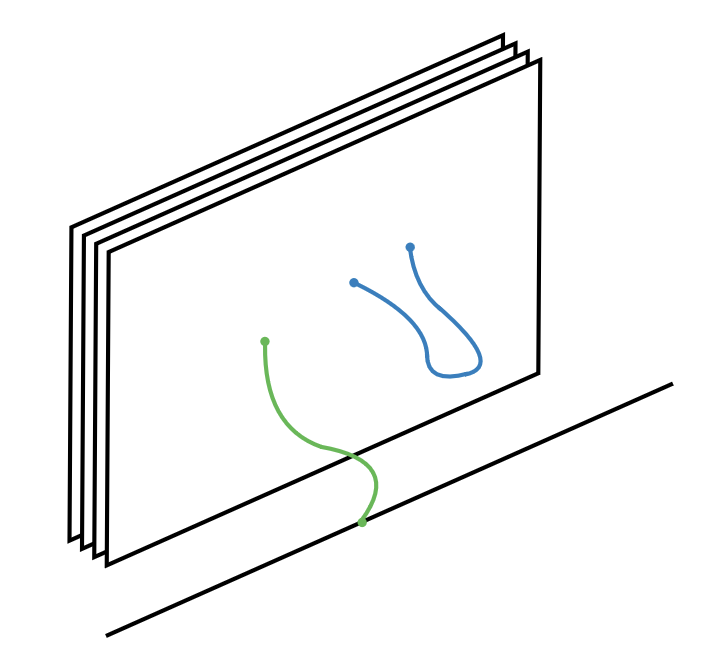
\includegraphics[width=0.5\textwidth]{IMAGES/brane-strings.png}
    \caption{Schematic representation of a stack of Dp branes and a single Dp' brane with strings attached. The blue string will have the same boundary conditions in all directions while the green string will have mixed conditions in some. Figure taken from \cite{Stemerdink:2022hnf}.}
    \label{fig:brane-schematic}
\end{figure}

As we did for the single D brane, the boundary conditions will lead to a relation between left and right moving modes. 

\begin{align}
    \text { NN: } X^\mu(z, \bar{z}) & =x^\mu-i \alpha^{\prime} p^\mu \ln (z \bar{z})+i \sqrt{\frac{\alpha^{\prime}}{2}} \sum_{m \neq 0} \frac{a_m^\mu}{m}\left(z^{-m}+\bar{z}^{-m}\right) \\
    \text { DN, ND: } X^\mu(z, \bar{z}) & =i \sqrt{\frac{\alpha^{\prime}}{2}} \sum_{r \in \mathbb{Z}+1 / 2} \frac{a_r^\mu}{r}\left(z^{-r} \pm \bar{z}^{-r}\right) \\
    \text { DD: } \quad X^\mu(z, \bar{z}) & =-i \frac{\delta X^\mu}{2 \pi} \ln (z / \bar{z})+i \sqrt{\frac{\alpha^{\prime}}{2}} \sum_{m \neq 0} \frac{a_m^\mu}{m}\left(z^{-m}-\bar{z}^{-m}\right)
\end{align}

Notice that the moding for the ND/DN directions gets shifted by $1/2$ to accomodate the mixed boundary conditions. This property is also apparent on the fermions 

Once again, we aim to calculate the massless spectrum. Thus, we want to find the zero point energy in both the R and the NS sector. As per usual, the R vacuum is massless, while the zero point energy for the NS sector is,

\begin{equation}
    \label{eq:zero-point-mixed}
    -\frac{1}{2} + \frac{\nu}{8}
\end{equation}

\section{D1/D5 spectrum}

The D1/D5 brane system will be the main example treated in this thesis. It deserves a propper introduction, so first of all let's define it in detail. Consider a stack of $Q_5$ D5 branes covering the 5, 6, 7, 8, 9 directions. Next, consider a stack of $Q_1$ D1 branes laying inside the D5 stack in the 5 direction. Table \ref{table:D1/D5} gives a summary of what was described.

\begin{table}[h]
    \centering
    \begin{tabular}{|l|l|l|l|l|l|l|l|l|l|l|}
    \hline
       & 0 & 1 & 2 & 3 & 4 & 5 & 6 & 7 & 8 & 9 \\ \hline
    D1 & - & . & . & . & . & - & . & . & . & . \\ \hline
    D5 & - & . & . & . & . & - & - & - & - & - \\ \hline
\end{tabular}
\caption{Schematic representation of the D1/D5 system.}
\label{table:D1/D5}
\end{table}

As we can see, the number of mixed directions is $\nu = 4$, so from equation \ref{eq:zero-point-mixed}, the zero point energy of the NS sector of 1-5 and 5-1 string vanishes. Then, the massless spectrum of excitations of these strings will be both the R vacuum and the NS vacuum. Take for instance a 1-5 string, meaning that the endpoint at $\sigma = 0$ lays in the D1 brane, while the one at $\sigma = \pi$ lays in the D5 brane. The bassless modes will be generated by,

\begin{align}
    \label{eq:zero-modes-d1d5}
    \text{NS: } &b_0^i, \quad i=6,7,8,9\\
    \text{R: }  &b_0^M, \quad M = 0,1,2,3,4,5
\end{align}

Both of these sectors generate Clifford algebras separately of the respective subgroups of $SO(1,9)$. At first glance, we could think the important subgroup is $SO(1,5) \times SO(4) \subset SO(1,9) $, but as it was mentionied previously, we want to focus on the theory on the intersection world-volume, so we want to look at the subgroup $SO(1,1) \times SO(4)_I \times SO(4)_E \subset SO(1,9)$, where the subindices indicate the directions 1, 2, 3, 4 for I and 6, 7, 8, 9 for E.

According to this splitting, the Clifford algebras of Equations \ref{eq:zero-modes-d1d5} generate spinors of $SO(1,5)$ and $SO(4)_I$ respectively. The $SO(1,5)$ spinor then splits into various $SO(1,1) \times SO(4)_E$ spinors.

Let's consider the R vacuum given by the $SO(1,5)$ spinor $\ket{s_0, s_1, s_2}$. The GSO projection picks one $SO(1,5)$ chirality, and in this case we decide it picks the $\mathbf{4}_s$.

We pick a basis where the first eigenvalue $s_0$ is associated to the 0, 5 directions, while the other are associated to the 1, 2, 3, 4 directions. This is convenient because the spinor splits as $\ket{s_0} \otimes \ket{s_1, s_2}$ under $SO(1,9) \rightarrow SO(1,1) \times SO(4)_E$. Now, counting chiralities in $SO(1,1)$ and $SO(4)_E$ we can see that this spinor fills the representations $(\mathbf{1}_s, \mathbf{2}_s) \oplus (\mathbf{1}_c, \mathbf{2}_c)$.

A similar, albeit easier calculation, shows that the NS vacuum is characterized by a $SO(4)_I$ spinor in the $\mathbf{2}_s$.

At last, the spectrum of the 1-5 string can be obtained by noticing that in the NS sector all states are $SO(4)_I$ singlets, while in the R sector they are $SO(1,1) \times SO(4)_E$ singlets, i.e,

\begin{align}
    \text{NS: } (\mathbf{1}_s, \mathbf{2}_s, \mathbf{1}) \oplus (\mathbf{1}_c, \mathbf{2}_c, \mathbf{1}) \\
    \text{R: } (\mathbf{1}, \mathbf{1}, \mathbf{2}_s)
\end{align}

Note that the 5-1 strings will produce the same zero modes, so that the vacuum will be identical.

The only missing piece at this point it the 1-1 and 5-5 massless spectrums. We already know that these come from the dimensional reduction of the $\mathbf{10}$ and the $\mathbf{16}_s$ of $SO(1,9)$. It is straight forward to see that the vector decomposes as $(\mathbf{2},\mathbf{1},\mathbf{1})\oplus(\mathbf{1},\mathbf{4},\mathbf{1}) \oplus(\mathbf{1},\mathbf{1},\mathbf{4})$. The procedure to decompose the spinor is very similar to what we did with the $\mathbf{4}_s$ of $SO(1,5)$ previously. Now we need to split the $\mathbf{16}_s$ via the eigenvalues $s_0$ in $SO(1,1)$, $s_1$, $s_2$ in $SO(4)_E$ and $s_3$, $s_4$ in $SO(4)_I$. Again, counting chiralities we end up with,

\begin{equation*}
    \mathbf{16}_s \rightarrow (\mathbf{1}_s, \mathbf{2}_s, \mathbf{2}_s) \oplus (\mathbf{1}_s, \mathbf{2}_c, \mathbf{2}_c) \oplus (\mathbf{1}_c, \mathbf{2}_c, \mathbf{2}_s) \oplus (\mathbf{1}_c, \mathbf{2}_s, \mathbf{2}_c)
\end{equation*}


\chapter{Orbifolds}
\label{chap:orbifold}
\pagestyle{fancy}

String theory can be defined on a vast number of different target spaces. String Theory on torus target spaces is an exactly solvable theory \cite{GREEN1983437}, but it does not produce phenomenologically plausible results for several reasons, including that tori preserve all supercharges of the noncompact background \cite{GrañaTriendl}.

Using orbifolds as target spaces, we fix this last issue because they can break supersymmetry \cite{Giaccari_2023}. The process can be throught of as gauging away global symmetries on the worldsheet in a way that the orbifolded spectrum is left with less supercharges than the original spectrum. This idea was first presented in \cite{DIXON1985678} in the special case of a toroidal orbifold. This specific type of orbifold will be the focus of this chapter.

In general, this argument makes orbifolds a good candidate for study as target spaces, and toroidal orbifolds are the first deviations we can make from plain torus compactification, making them the easiest examples to work explicitly.

\section{Orbifold compactification}

We are interested in compactifications of the type,

\begin{equation}
    \mathbb{R}^{1,4} \times S^1 \times T^4.
\end{equation}

Consider the worldsheet scalars $X^M = (X^\mu, Z, Y^m)$ split according to the decomposition of the target space above $M = 0,\dots,9$, $\mu = 0,1,2,3,4$, $m = 1,2,3,4$. We can arrange the torus scalars as,

\begin{equation}
    \label{eq:4_complex_torus}
    W^i=\frac1{\sqrt{2}}(Y^{2i-1}+iY^{2i}),\quad i=1,2.
\end{equation}

The torus structure is contained in each complex torus coordinate as an identification of the type $W^i \sim W^i + 1 \sim W^i + \tau^i$ for some $\tau \in \mathbb{C}$. The equations of motion for these scalars allow us to split them into left and right movers as,

\begin{equation}
    W^i(\tau,\sigma)=W_{L}^i(\tau+\sigma)+W_{R}^i(\tau-\sigma).
\end{equation}

It is now apparent that there can be 4 independent $\mathbb{Z}_p$ rotations acting on each of the torus coordinates that we have split into right and left movers.

\begin{equation}
    \label{eq:4_scalar_orb_action}
    \begin{gathered}
W_{L}^{1}\rightarrow e^{2\pi iu_{1}/p}W_{L}^{1} \\
W_{R}^{1}\rightarrow e^{2\pi iu_{2}/p}W_{R}^{1} \\
W_{L}^{2}\rightarrow e^{2\pi iu_{3}/p}W_{L}^{2} \\
W_{R}^2\to e^{2\pi iu_4/p}W_{R}^2, 
\end{gathered}
\end{equation}

The $S^1$ coordinate will be identified with a shift, $Z \sim Z+2\pi r/p$, making the  orbifold freely acting.

This story is not complete, as we should have introduced the discrete symmetry as a subgroup of the T-duality of the 4-torus $SO(4,4\mathbb{Z})$ and chosen the integers $u_i$ accordingly to suit the rotational subgroups of the T-duality group. The details are contained in \cite{gkountoumis2023freely,Stemerdink:2022hnf}, and the integers are characterized by mass parameter $m_i$,

\begin{align}
    \frac{2\pi u_1}p=m_1+m_3,\quad\frac{2\pi u_2}p=m_2+m_4\\\frac{2\pi u_3}p=m_1-m_3,\quad\frac{2\pi u_4}p=m_2-m_4.
\end{align}

Notice that the mass parameters may not be equal in certain cases. When the right movers and left movers are rotated in unequivalent ways, we refer to the space as an asymmetric orbifold. When they rotate in the same way though, we refer to those as symmetric orifolds.

Only some values of $p$ are actually permited for 4-tori. In our case, we want to restrict to orbifolds that can preserve some supercharges, so we restrict to $p = 2,3,4,6$.

In order to fully characterize the action of the orbifold on the spectrum of the superstring, we still need to know the charges of the fermionic modes and of the R vacuum (the NS vacuum is a scalar so it is uncharged by definition). The first is straight forward, because they tansform the same way as the scalar modes by supersymmetry. The latter requires a bit of extra work.

Take a basis element $\ket{s_0, s_1, s_2, s_3, s_4}_{L/R}$ of the R vacuum. The eigenvalues $s_i$, $i = 1,2,3,4$, by construction, are eigenvalues of the $SO(2)$ rotations of the plane $(2i+1,2i+2)$. Since the orbifold acts precisely as separate discrete subgroups of these $SO(2)$ rotations for both left and right movers, we can conclude that,

\begin{align}
    \ket{s_0,s_1,s_2,s_3,s_4}_{L} \rightarrow  e^{2\pi i (\tilde{u}_1 s_3 + \tilde{u}_2 s_4)}\ket{s_0,s_1,s_2,s_3,s_4}_{L}\\
    \ket{s_0,s_1,s_2,s_3,s_4}_{R} \rightarrow e^{2\pi i (\tilde{u}_3 s_3 + \tilde{u}_4 s_4)} \ket{s_0,s_1,s_2,s_3,s_4}_{R}
\end{align}

Looking at the charges of the scalars, we can read that,

\begin{align}
    \tilde{u}_{3}=\frac{m_{1}+m_{3}}{2\pi},u_{3}=\frac{m_{2}+m_{4}}{2\pi},\\\tilde{u}_{4}=\frac{m_{1}-m_{3}}{2\pi},u_{4}=\frac{m_{2}-m_{4}}{2\pi}.
\end{align}

The classification is complete if we specify values for $(s_3, s_4)$, for a left moving vacuum the charges are,

\begin{align}
    (+1/2, +1/2) : m_1,\\
    (+1/2, -1/2) : -m_1,\\
    (-1/2, +1/2) : m_3,\\
    (-1/2, -1/2) : -m_3,
\end{align}

while for a right moving vacuum they are,

\begin{align}
    (+1/2, +1/2) : m_2\\
    (+1/2, -1/2) : -m_2\\
    (-1/2, +1/2) : m_4\\
    (-1/2, -1/2) : -m_4
\end{align}

We can notice that only 2 aspects mattered to find out how all these objects were charged by the orbifold action. Firstly, we need to know if it is left or right moving. Secondly, since it acts as rotations in the $SO(4)$ subgroup related to the torus directions of the Lorentz group $SO(1,9)$, we only need to know in which representation of the Lorentz group an object sits, and we will automatically know how it is charged by the orbifold action.

\begin{table}[h]
    \centering
    \begin{tabular}{cccc}
    Sector              & State                          & L charge     & R charge     \\ \hline
    \multirow{4}{*}{NS} & $b_{-1/2}^1\ket{0}$            & $m_1+m_3$    & $m_2+m_4$    \\
                        & $\overline{b}_{-1/2}^1\ket{0}$ & $-(m_1+m_3)$ & $-(m_2+m_4)$ \\
                        & $b_{-1/2}^2\ket{0}$            & $m_1-m_3$    & $m_2-m_4$    \\
                        & $\overline{b}_{-1/2}^2\ket{0}$ & $-(m_1-m_3)$ & $-(m_2-m_4)$ \\ \hline
    \multirow{4}{*}{R}  & $\ket{s_0,s_1,s_2,+1/2,+1/2}$  & $m_1$        & $m_2$        \\
                        & $\ket{s_0,s_1,s_2,-1/2,-1/2}$  & $-m_1$       & $-m_2$       \\
                        & $\ket{s_0,s_1,s_2,-1/2,+1/2}$  & $m_3$        & $m_4$        \\
                        & $\ket{s_0,s_1,s_2,-1/2,-1/2}$  & $-m_3$       & $-m_4$      
\end{tabular}
\end{table}

It is more useful for this thesis to organize all these objects as representations of $SO(2)\times SO(2) \subset SO(4)$. The bosonic part comes from a $\mathbf{4}$ of $SO(4)$, and it splits into $(\mathbf{2},\mathbf{1}) \oplus (\mathbf{1},\mathbf{2})$ of $SO(2)\times SO(2)$. Just to make it explicit, take \ref{eq:4_complex_torus}, we have,

\begin{align}
    Y^1_L = \frac{1}{\sqrt{2}} (W^1_L + \overline{W^1}_L) \\
    Y^2_L = \frac{1}{\sqrt{2i}} (W^1_L - \overline{W^1}_L) 
\end{align}

The charges of the complex torus coordinates lead us to just a usual $SO(2)$ rotation,

\begin{equation}
    \begin{bmatrix}Y_L^1\\Y_L^2\end{bmatrix}\to\begin{bmatrix}\cos{(m_1+m_3)}&&-\sin{(m_1+m_3)}\\\sin{(m_1+m_3)}&&\cos{(m_1+m_3)}\end{bmatrix}\begin{bmatrix}Y_L^1\\Y_L^2\end{bmatrix}
\end{equation}

An equivalent calculation with $W^2$ leads to the same rotation but with the respective charges for the real coordinates $(Y^3, Y^4)$. We could read this from the table from the fact that the charges present themselves in the same linear combination for each $SU(2)$ vector. For the spinors, a similar phenomenom happens.

We now can arrange the spinors into chiral representations of $SO(4)$. Take for instance the components  with charge $m_1$, they can be arranged into the $\mathbf{2}_s$ of $SO(4)$. The other half of the spinor, with charge $m_3$ forms a $\mathbf{2}_c$ of $SO(4)$.

\begin{table}[h]
    \label{table:superimportant_orbifold_charges}
    \centering
    \begin{tabular}{ccc}
    SO(4) rep                 & L charge  & R charge  \\ \hline
    $(\mathbf{2},\mathbf{1})$ & $m_1+m_3$ & $m_2+m_4$ \\
    $(\mathbf{1},\mathbf{2})$ & $m_1-m_3$ & $m_2-m_4$ \\ \hline
    $\mathbf{2}_s$            & $m_1$     & $m_2$     \\
    $\mathbf{2}_c$            & $m_3$     & $m_4$    
\end{tabular}
\caption{Orbifold charges for relevant representations of the subgroup of the Lorentz group corresponding to the torus $SO(4)\subset SO(1,9)$.}
\end{table}

Usualy, vectors of $SO(4)$ will not be split into their $SO(2)\times SO(2)$ components unless $m_1 = m_2 = m_3 = m_4 \neq 0$.


\section{Branes in orbifold backgrounds}

Building D-branes on orbifold backgrounds is not as easy as one could have expected. The orbifold action may break the boundary conditions of the open strings attached to the D-brane, forbidding it from existing in the theory. As we will se in the following, both the D1 and D5 branes we are interested in can survive if we restrict our study to symmetric orbifolds.

First of all, consider the general scenario of a single D brane as discussed in \ref{sec:pre_branes}. We introduced the conditions on the open string modes that enable us to define D-branes,

\begin{equation}
    a^a = \tilde{a}^a,
\end{equation}

if the boundary conditions were Neumann, or

\begin{equation}
    a^i = -\tilde{a}^i,
\end{equation}

if they were Dirichlet. The $a$ and $i$ indices are in the vector representation of the corresponding subgroups of $SO(1,9)$. The D-brane corresponding to these boundary conditions will be able to exist in the orbifold background if said conditions are respected by the orbifold group action.

As the orbifold group only charges the $T^4$ directions, we can restrict the study the boundary conditions on these directions. First of all, taking from the complex coordinate definition \ref{eq:4_complex_torus}, we define the modes,

\begin{align}
    w^i = \frac{1}{\sqrt{2}} (a^{2i-1} + i a^{2i}) \\
    \tilde{w}^1 = \frac{1}{\sqrt{2}} (\tilde{a}^{2i-1} + i \tilde{a}^{2i})
\end{align}

The orbifold action on this complex modes is as in \ref{eq:4_scalar_orb_action},

\begin{equation}
    \begin{aligned}
        w^i \rightarrow e^{i(m_1 \pm m_3)} w^1\\
        \tilde{w}^1 \rightarrow e^{i(m_2 \pm m_4)} \tilde{w}^1
    \end{aligned}
\end{equation}
where the $i = 1$ takes the $+$, and $i = 2$, the $-$ signs.

Now, take for instance the first complex coordinate $w^1$ and $\tilde{w}^1$. If the brane we wanted to construct had only N or D conditions on this $T^2$, say $a^1  = \pm \tilde{a}^1$ and $a^2 = \pm \tilde{a}^2$, this translates as $w^1 = \pm \tilde{w}^1$. In the other hand, if we had mixed conditions on these directions, $a^1 = \pm \tilde{a}^1$ and $a^2 = \mp \tilde{a}^2$, they would imply $\overline{w}^1 = \pm\tilde{w}^1$.\footnote{The overline represents complex conjugation.}

Since the orbifold action is a phase on the complex modes, the only difference between different brane constructions will be if they imply complex conjugation in the boundary conditions. This leads to essentially 4 different cases that we can treat without loss of generality.

\textbf{Case 1: } $w^1 = \tilde{w}^1$ and $w^2 = \tilde{w}^2$. The group action on these conditions is,

\begin{equation}
    \begin{cases}
        e^{i(m_1 + m_3)} w^1 = e^{i(m_2 + m_4)} \tilde{w}^1 \\
        e^{i(m_1 - m_3)} w^2 = e^{i(m_2 - m_4)} \tilde{w}^2
    \end{cases}
\end{equation}

From which we extract the condition on the mass parameters,

\begin{equation}
    \begin{cases}
        m_1 = m_2 \\
        m_3 = m_4
    \end{cases}
\end{equation}

This is what is known as a symmetric orbifold, one in which left and right movers are rotated in the same manner. The D1 and D5 branes defined in \ref{tab:3_d1d5_definition} are examples that follow this case.

\textbf{Case 2: } $\overline{w}^1 = \tilde{w}^1$ and $\overline{w}^2 = \tilde{w}^2$. The group action on these conditions is,

\begin{equation}
    \begin{cases}
        e^{-i(m_1 + m_3)} \overline{w}^1 = e^{i(m_2 + m_4)} \tilde{w}^1 \\
        e^{-i(m_1 - m_3)} \overline{w}^2 = e^{i(m_2 - m_4)} \tilde{w}^2
    \end{cases}
\end{equation}

From which we extract the condition on the mass parameters,

\begin{equation}
    \begin{cases}
        m_1 = -m_2 \\
        m_3 = -m_4
    \end{cases}
\end{equation}
This kind of orbifold is usually called anti-symmetric, in the sense that the right movers rotate in the oposite direction of the left movers.

The last two cases are not particularly useful for this thesis but are left here for the sake of completeness. There is, as far as I know, no special name for the orbifolds that allow these kinds of branes.

\textbf{Case 3: } $w^1 = \tilde{w}^1$ and $\overline{w}^2 = \tilde{w}^2$. The group action on these conditions is,

\begin{equation}
    \begin{cases}
        e^{i(m_1 + m_3)} w^1 = e^{i(m_2 + m_4)} \tilde{w}^1 \\
        e^{-i(m_1 - m_3)} \overline{w}^2 = e^{i(m_2 - m_4)} \tilde{w}^2
    \end{cases}
\end{equation}

From which we extract the condition on the mass parameters,

\begin{equation}
    \begin{cases}
        m_1 = m_4 \\
        m_2 = m_3
    \end{cases}
\end{equation}

\textbf{Case 4: } $\overline{w}^1 = \tilde{w}^1$ and $w^2 = \tilde{w}^2$. The group action on these conditions is,

\begin{equation}
    \begin{cases}
        e^{-i(m_1 + m_3)} \overline{w}^1 = e^{i(m_2 + m_4)} \tilde{w}^1 \\
        e^{i(m_1 - m_3)} w^2 = e^{i(m_2 - m_4)} \tilde{w}^2
    \end{cases}
\end{equation}

From which we extract the condition on the mass parameters,

\begin{equation}
    \begin{cases}
        m_1 = -m_4 \\
        m_2 = -m_3
    \end{cases}
\end{equation}

In the following section we will study in more detail the D1/D5 system defined in \ref{tab:3_d1d5_definition}, and as we have seen in \textbf{Case 1}, only symmetric orbifolds allow the existence of the system. We will restrict to $m_1 = m_2$ and $m_3 = m_4$ for the rest of the thesis.

\section{Orbifold group action on the spectrum of the D1/D5 system}

The effect of orbifolding on the spectrum of a theory projects out states that are not invariant under the orbifold action, gauging away the global symmetry that defined the orbifold in the first place \cite{Giaccari_2023}. It was discovered that for freely acting orbifolds, this process happens through a Higgs-like mechanism that gives mass to states charged under the obrifold action \cite{gkountoumis2023freely} (thus the name \textit{mass parameters}).

In this section we will study the resulting spectrum of the D1/D5 system defined in \ref{tab:3_d1d5_definition} after orbifolding the target space. The remaining field content will lead us to discover the amount of supercharges in the orbifolded theory, from which we will read and classify the supersymmetry breaking for different orbifolds.

Firstly, let us summarize the results of section \ref{sec:D1D5_spectrum}. Note that all representations labeled as $(\cdot, \cdot, \cdot)$ are representing the $SO(1,1) \times SO(4)_E \times SO(4)_I$ representations in that order.

\begin{table}[h]
\label{tab:4_d1d5_spectrum}
    \begin{tabular}{lc|c|c}
                                                          & 1-1 strings                                       & 5-5 strings                                       & 1-5 strings                                  \\ \hline
    \multicolumn{1}{l|}{Bosonic}                    & $(2,1,1)+(1,4,1)+(1,1,4)$                         & $(2,1,1)+(1,4,1)+(1,1,4)$                         & $2(1,1,2_s)$                                  \\ \hline
    \multicolumn{1}{l|}{\multirow{2}{*}{Fermionic}} & $(1_s,2_s,2_s)+(1_s,2_c,2_c)+$                    & $(1_s,2_s,2_s)+(1_s,2_c,2_c)+$                    & \multirow{2}{*}{$2(1_s,2_s,1)+2(1_c,2_c,1)$} \\
    \multicolumn{1}{l|}{}                                 & \multicolumn{1}{l|}{$(1_c,2_s,2_c)+(1_c,2_c,2_s)$} & \multicolumn{1}{l|}{$(1_c,2_s,2_c)+(1_c,2_c,2_s)$} &                                             
\end{tabular}
\caption{Massless spectrum of the D1/D5 system before projecting charged states.}
\end{table}

\textbf{Case 1: } $m_i = 0$, corresponds to the spectrum in \ref{tab:4_d1d5_spectrum}, so the spectrum has $\mathcal{N} = (4,4)$ supercharges.

\textbf{Case 2: } $m_1 = m_2 = 0$ and $m_3 = m_4 \neq 0$. In this case, all representations containing the $\mathbf{2}_c$ or $\mathbf{4}$ of $SO(4)_I$ are projected out. This projection leads to the following spectrum,

\begin{table}[h]
    \centering
    \begin{tabular}{lc|c|c}
                                   & 1-1 strings                   & 5-5 strings                   & 1-5 strings                 \\ \hline
    \multicolumn{1}{l|}{Bosonic}   & $(2,1,1)+(1,4,1)$             & $(2,1,1)+(1,4,1)$             & $2(1,1,2_s)$                \\ \hline
    \multicolumn{1}{l|}{Fermionic} & $(1_s,2_s,2_s)+(1_c,2_c,2_s)$ & $(1_s,2_s,2_s)+(1_c,2_c,2_s)$ & $2(1_s,2_s,1)+2(1_c,2_c,1)$
\end{tabular}
\end{table}

Counting states in each sector of the spectrum we see that supersymmetry can still be present and indeed the field content is compatible with $(4,4)$ supersymmetry, implying that even if some fields were projected away, all supercharges can remain in the theory.

\textbf{Case 3: } $m_1 = m_2 \neq 0$ and $m_3 = m_4 = 0$. This case is similar to the previous but now the $\mathbf{2}_c$ survives, and the $\mathbf{2}_s$ is the one projeted out.

\begin{table}[h]
    \centering
    \begin{tabular}{lc|c|c}
                                   & 1-1 strings                   & 5-5 strings                   & 1-5 strings                 \\ \hline
    \multicolumn{1}{l|}{Bosonic}   & $(2,1,1)+(1,4,1)$             & $(2,1,1)+(1,4,1)$             & -                \\ \hline
    \multicolumn{1}{l|}{Fermionic} & $(1_s,2_c,2_c)+(1_c,2_c,2_c)$ & $(1_s,2_c,2_c)+(1_c,2_c,2_c)$ & $2(1_s,2_s,1)+2(1_c,2_c,1)$
\end{tabular}
\end{table}

In this case, just looking at the 1-5 sector we notice that only fermions survive. This is a clear indication that all supercharges were broken, as the superpartners of the 1-5 fermions are not in the spectrum anymore. The remaining supercharges are $\mathcal{N} = (0,0)$.

\textbf{Case 3.1: } $m_1 = m_2 \neq 0$ and $m_3 = m_4 \neq 0$, with $m_1 \neq m_3$. In this case, every object that is not a singlet under $SO(4)_I$ is charged under the orbifold action.

\begin{table}[h]
    \centering
    \begin{tabular}{lc|c|c}
                                   & 1-1 strings                   & 5-5 strings                   & 1-5 strings                 \\ \hline
    \multicolumn{1}{l|}{Bosonic}   & $(2,1,1)+(1,4,1)$             & $(2,1,1)+(1,4,1)$             & -                \\ \hline
    \multicolumn{1}{l|}{Fermionic} & - & - & $2(1_s,2_s,1)+2(1_c,2_c,1)$
\end{tabular}
\end{table}

It is clear again that no supercharges remain in the theory. It was always expected that turning all the mass parameters would break all supersymmetry as it was already known for the closed string.

\textbf{Case 3.2: } $m_1 = m_2 = m_3 = m_4 \neq 0$. In thi special case when all parameters are aqual, we see that we should split the representations according to $SO(2) \times SO(2) \subset SO(4)_I$. In this special case, half of the $\mathbf{4}$ of $SO(4)_I$ is uncharged.

\begin{table}[h]
    \centering
    \begin{tabular}{lc|c|c}
                                   & 1-1 strings                   & 5-5 strings                   & 1-5 strings                 \\ \hline
    \multicolumn{1}{l|}{Bosonic}   & $(2,1,1)+(1,4,1) + (1,1,(1,2))$             & $(2,1,1)+(1,4,1)$             & -                \\ \hline
    \multicolumn{1}{l|}{Fermionic} & - & - & $2(1_s,2_s,1)+2(1_c,2_c,1)$
\end{tabular}
\end{table}

Although the field content is enlarged in this case compared to the previous, again all supersymmetry is broken to $\mathcal{N} = (0,0)$.


%%%%%%%%%%%%%%%%%%%%%%%%%%%%%%%%%%%%%%%%%%%%%%%%%%
%%%%		~~~~ Conclusions ~~~~
%%%%%%%%%%%%%%%%%%%%%%%%%%%%%%%%%%%%%%%%%%%%%%%%%%


\chapter{D-brane gauge theories}
\label{chap:conclusion}
\pagestyle{fancy}

\section{Gauge theory on a single brane and dimensional reduction}

\section{Gauge theory of the D1/D5 system}

\section{Coulomb and Higgs branch}

\chapter{Infrared limit and Black Hole thermodynamics}
\label{infrared}
\pagestyle{fancy}

\section{IR SCFT = black hole theormodynamics}

\section{Predictions of IR limit in orbifold context}
\chapter{Conclusions}
\label{chap:conclusions}
\pagestyle{fancy}



%%%%%%%%%%%%%%%%%%%%%%%%%%%%%%%%%%%%%%%%%%%%%%%%%%
%%%%		~~~~ START DOCUMENT: Backmatter ~~~~
%%%%%%%%%%%%%%%%%%%%%%%%%%%%%%%%%%%%%%%%%%%%%%%%%%



\newpage
% SETTING FOR APPENDIX ENVIRONMENT
{
\begin{LARGE}
\textbf{Appendices}
\end{LARGE}\\
\noappendicestocpagenum
\renewcommand{\appendixtocname}{Appendix}
\renewcommand{\appendixpagename}{Appendix}
\appendix
\addappheadtotoc
\normalsize
}
\appendix

% APPENDIX
\chapter{Spinors in various dimensions}
\label{ap:spinors}

In this appendix we will juntify some claims about spinors in general even dimensions that are used throughout the thesis.

It is well known that the Dirac representation is not irreducible in even dimensions, in which a chirality projection exists into the two different Weyl basis. There is also always a Majorana condition that can induces a real structure in the spinor spaces of all dimensions, but is only truncates the degrees of freedom of Weyl spinors in some dimensions. All these topics will be covered in the following sections in detail with the main objective of describing irreducible spinors in all even dimensions $D \leq 10$.

% START APPENDIX
\section{Weyl Spinors in $D = 2,4,6,8,10$}

We start with the Clifford algebra,

\begin{equation}
    \label{eq:cliff_alg}
    \{ \Gamma^\mu, \Gamma^\nu \} = 2\eta^{\mu \nu},
\end{equation}

and let the metric be $\eta^{\mu \nu} = \text{diag}\left( -1,1,\dots,1 \right)$ the $D = 2k + 2$ dimensional Minkowski metric.

We first make a change of basis for the algebra elements so that the fundamental representation can be directly extracted from the algebra. Take the following linear combinations,

\begin{align}
    \label{eq:cliff_rebase}
    & \Gamma^{0 \pm}=\frac{1}{2}\left( \pm \Gamma^0+\Gamma^1\right) \\
    & \Gamma^{a \pm}=\frac{1}{2}\left(\Gamma^{2 a} \pm i \Gamma^{2 a+1}\right), \quad a=1, \ldots, k
\end{align}

Now the Clifford algebra \ref{eq:cliff_alg} can be stated in terms of the new operators as,

\begin{equation}
    \begin{aligned}
    & \left\{\Gamma^{a+}, \Gamma^{b-}\right\}=\delta^{a b} \\
    & \left\{\Gamma^{a+}, \Gamma^{b+}\right\}=\left\{\Gamma^{a-}, \Gamma^{b-}\right\}=0 .
    \end{aligned}
\end{equation}

We can see that these operators are raising and lowering operators for $k+1$ different eigenvalues. We can write an arbitrary basis element of this representation as $\ket{s_0, \dots, s_{k}}$, with $s_i = \pm 1$. An arbitrary spinor in this representation is then in the complex span of this basis, which has $2^{k+1}$ complex components. This is what is called a Dirac spinor, or $\mathbf{2^{k+1}}_{\text{Dirac}}$.

These eigenvalues $s_i$ are actually eigenvalues of rotations in planes given by the grouping of \ref{eq:cliff_rebase}. To see this explicitly, we need to recover the Lorentz algebra from the Clifford algebra. Define,

\begin{equation}
    \Sigma^{\mu v}=-\frac{i}{4}\left[\Gamma^\mu, \Gamma^v\right]
\end{equation}

The elements $\Sigma^{\mu v}$ define the Lorentz algebra os $SO(1, 2k+1)$. The generators $\Sigma^{2a,2a+1}$ commute and have eigenvalues proportional to $s_a$ when acting on the basis element $\ket{s_0, \dots, s_{k}}$. To be precise, the operator,

\begin{equation}
    S_a \equiv i^{\delta_{a, 0}} \Sigma^{2 a, 2 a+1}=\Gamma^{a+} \Gamma^{a-}-\frac{1}{2}
\end{equation}

has eigenvalue $s_a$.

Next, we can define the chirality operator,

\begin{equation}
    \label{eq:chirality_op}
    \Gamma=i^{-k} \Gamma^0 \Gamma^1 \ldots \Gamma^{d-1}
\end{equation}

which has the properties,

\begin{equation}
    (\Gamma)^2=1, \quad\left\{\Gamma, \Gamma^\mu\right\}=0, \quad\left[\Gamma, \Sigma^{\mu v}\right]=0
\end{equation}

From the first property, we see that $\Gamma$ has eigenvalues $\pm 1$. From the rest we see that we can split the basis $\ket{s_0,\dots,s_k}$ into two subspaces according to the eigenvalues of $\Gamma$. We can rewrite the chirality operator in terms of the rotation generators $S_a$ as follows,

\begin{equation}
    \Gamma=2^{k+1} S_0 S_1 \ldots S_k
\end{equation}

which allows us to identify the two chiralities as $+1$ when the product of the $s_a$ is positive and $-1$ when it is negative. The two subspaces defined by the chirality operator are called Weyl representations and are labeled as $\mathbf{2^k}_s$ and $\mathbf{2^k}_c$ for the $+1$ and $-1$ subspaces respectively. So we can finally state that the dirac representation splits into Weyl representations as,

\begin{equation}
    \mathbf{2^{k+1}}_\text{Dirac} = \mathbf{2^k}_s \oplus \mathbf{2^k}_c
\end{equation}

\section{Majorana condition}

\section{Table of irreducible spinors in even dimensions}


% BIBLIOGRAPHY
\setstretch{1} % DECREASE LINE SPACING IN BIBLIOGRAPHY
\normalsize\printbibliography[title={Bibliography}]
\addcontentsline{toc}{chapter}{Bibliography} \markboth{Bibliography}{Bibliography}


% END DOCUMENT
\end{document}
